\documentclass[a4paper]{article}

%document
\usepackage[top=10pt,bottom=10pt,left=10pt,right=10pt]{geometry}
\usepackage{layout}

%math
\usepackage{mathtools}
\usepackage{amsmath}
\usepackage{amssymb}
\usepackage{amsfonts}

%tikzpicture
\usepackage{tikz}
\usepackage{scalerel}
\usepackage{pict2e}
\usepackage{tkz-euclide}
\usetikzlibrary{calc}
\usetikzlibrary{patterns,arrows.meta}
\usetikzlibrary{shadows}
\usetikzlibrary{external}
\usetikzlibrary{positioning}

%pgfplots
\usepackage{pgfplots}
\pgfplotsset{compat=newest}
\usepgfplotslibrary{statistics}
\usepgfplotslibrary{fillbetween}

%colours
\usepackage{xcolor}
\pagenumbering{gobble}

\begin{document}	
	\layout
	
	\begin{enumerate}
		\item Make 3 styles.
		\item Style 1 is called ``A''.
		\item Style 2 is called ``B''.
		\item Style 3 is called ``C''.
	\end{enumerate}
	
	\begin{center}
		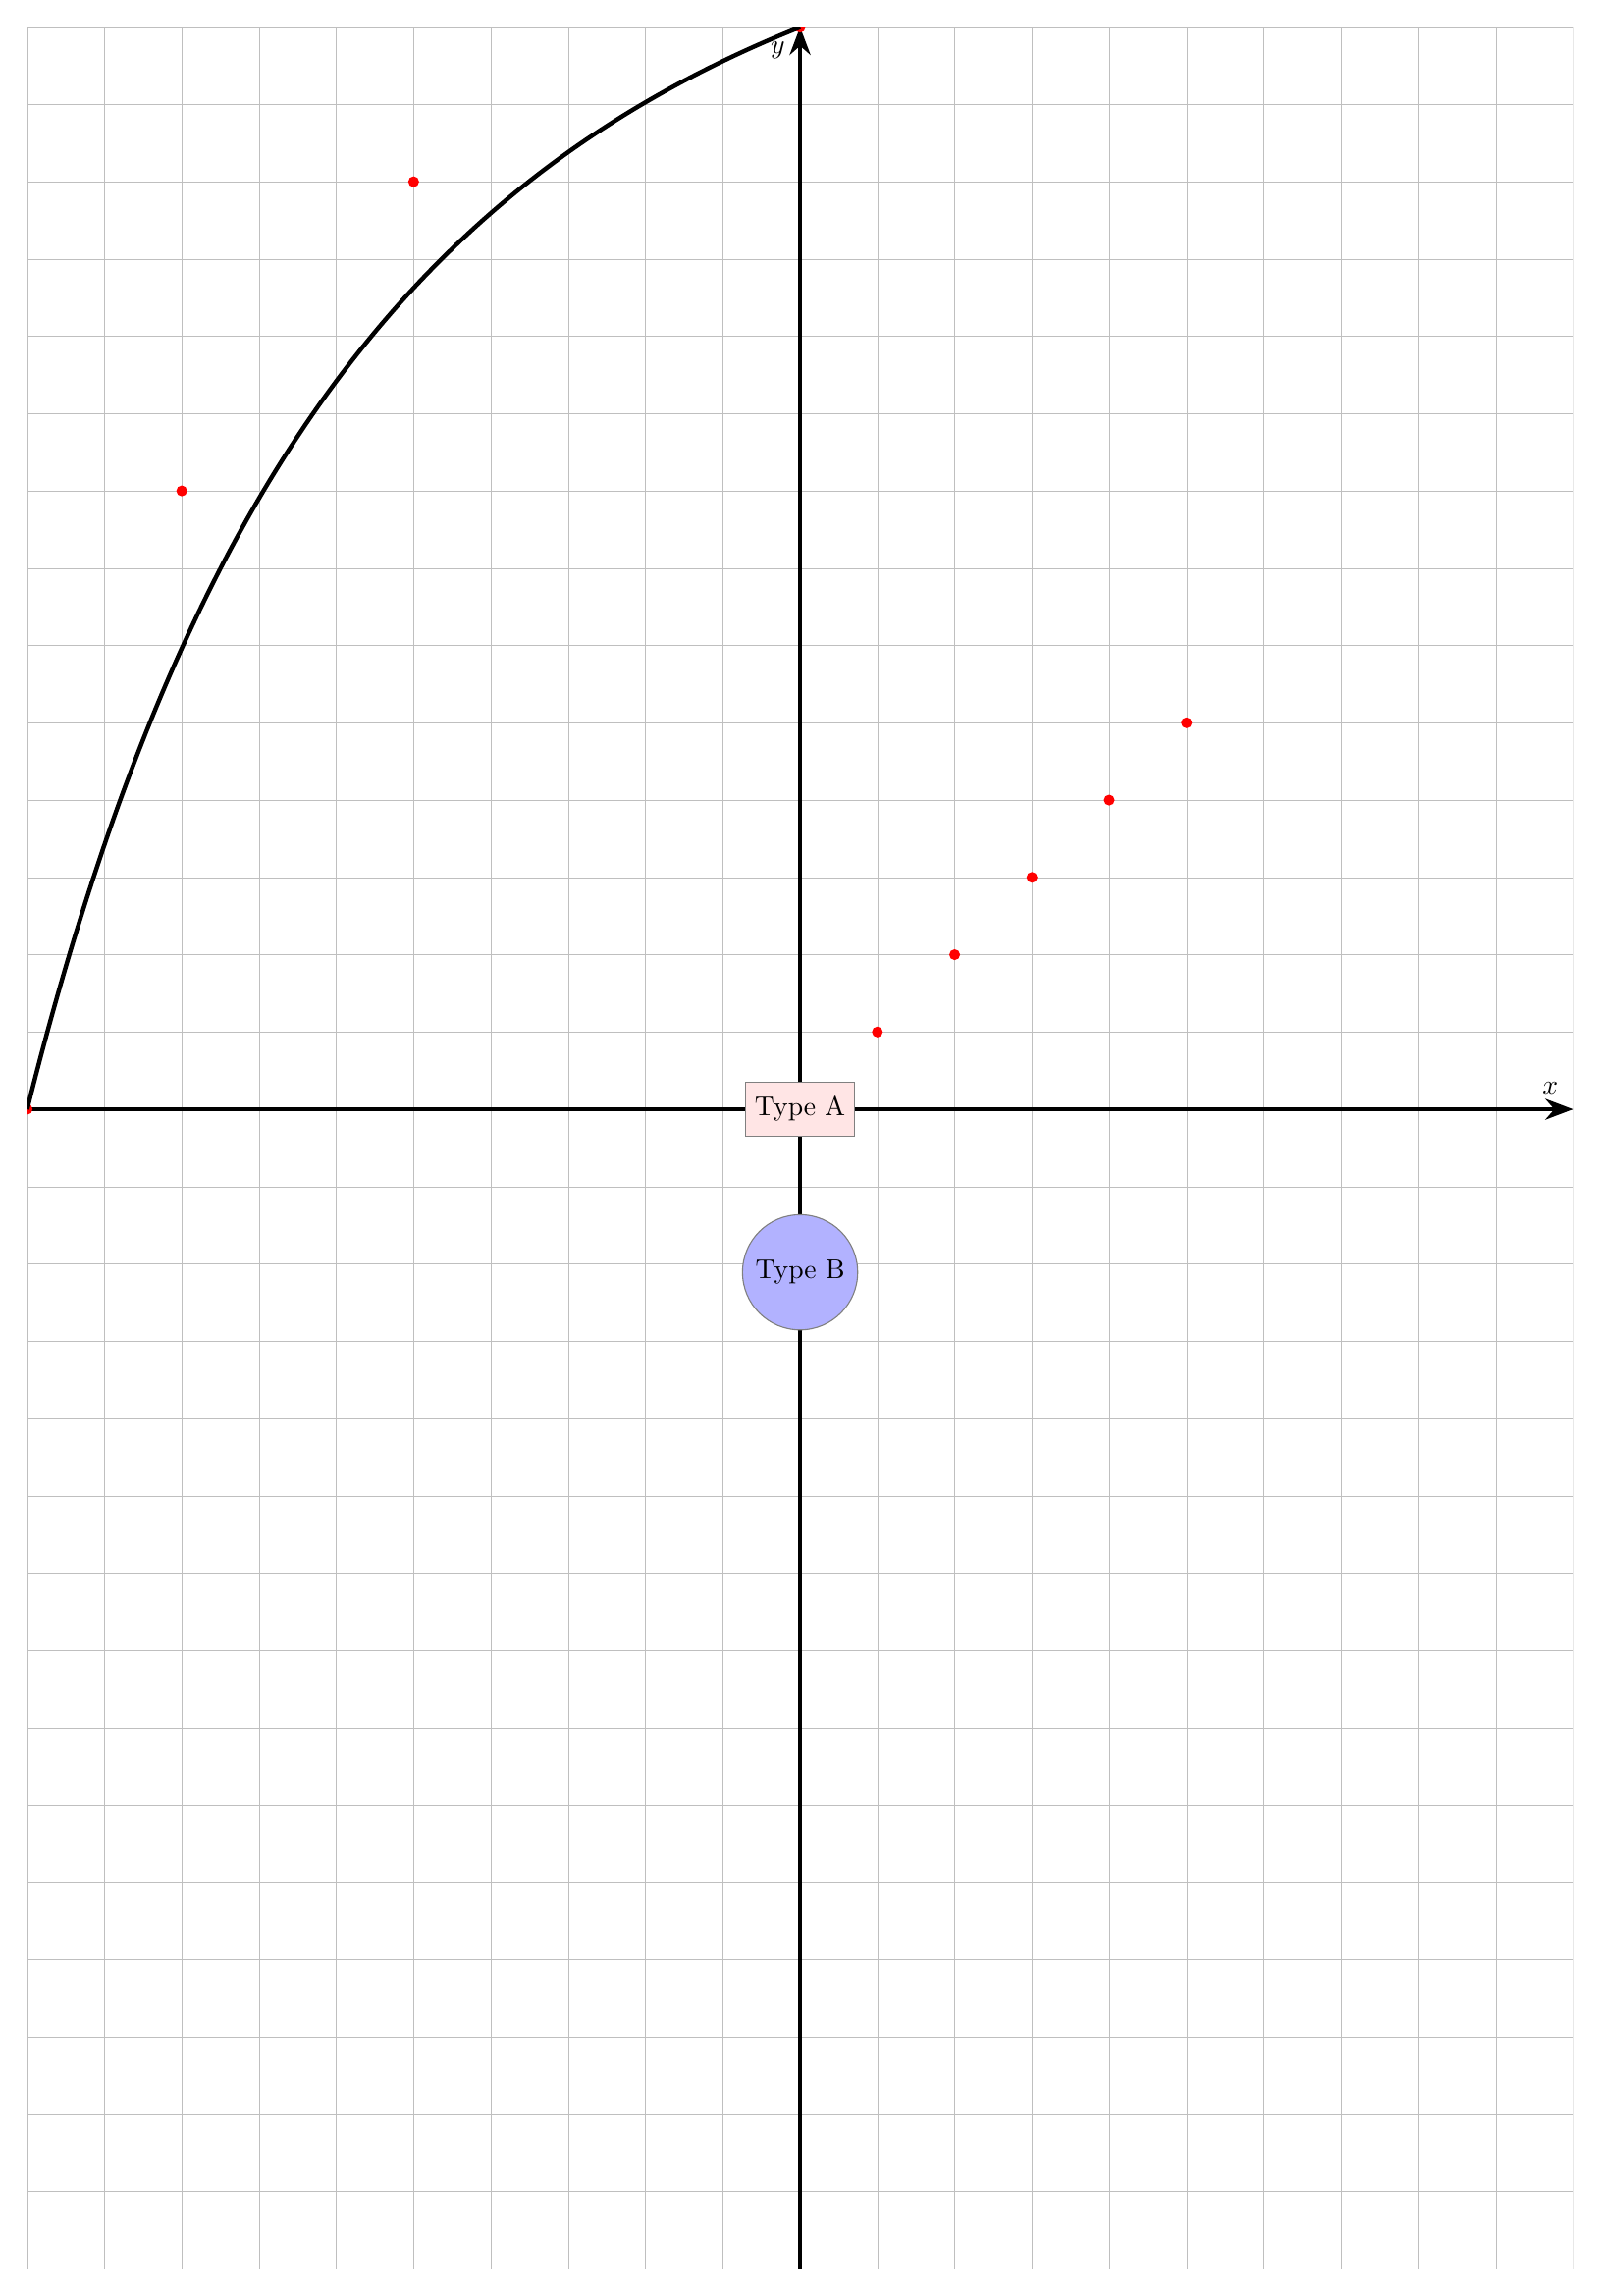
\begin{tikzpicture}[
			A/.style={rectangle,draw=black!50,fill=red!10,minimum size=7mm},	
			B/.style={circle,draw=black!50,fill=blue!30,minimum size=7mm},
			]		
			
			%clip
			\clip (-10,-15) rectangle (10,14);
			%grid
			\draw[lightgray,step=1,ultra thin] (-10,-15) grid (10,14);
		
			%x-axis
			\draw[ultra thick,-Stealth] (-10,0)--(10,0) node[above left=2pt] {$x$};
			%y-axis
			\draw[ultra thick,-Stealth] (0,-15)--(0,14) node[below left=2pt]{$y$};
		
			\fill[red] (-10,0) circle (2pt);
			\fill[red] (-8,8) circle (2pt);
			\fill[red] (-5,12) circle (2pt);
			\fill[red] (0,14) circle (2pt);
			
			\draw[ultra thick] (-10,0) .. controls (-8,8) and (-5,12) .. (0,14);	
			
			\foreach \x in {0,1,2,3,4,5} 
			{
				\fill[color=red] (\x,\x) circle (2pt);
			}
			
			\node[A] (First) {Type A};
			\node[B] (Second) [below=of First] {Type B};
			
								
		
	\end{tikzpicture}
	
	
	
\end{center}	
	
\end{document}
